\documentclass[11pt]{article}

% ================================================================ packages
\usepackage{lmodern}
\usepackage[T1]{fontenc}
\usepackage[utf8]{inputenc}
\usepackage[margin=1in]{geometry}
\usepackage{amsmath,amssymb}
\usepackage{booktabs,longtable,array}
\usepackage{graphicx}
\usepackage{xcolor}
\usepackage{microtype}
\usepackage{enumitem}
\usepackage[most]{tcolorbox}
\usepackage{titlesec}
\usepackage{listings}
\usepackage{fancyhdr}
\usepackage{caption}
\usepackage{float}
\usepackage{tikz}
\usetikzlibrary{arrows.meta,positioning,calc,fit,backgrounds}
\usepackage[colorlinks=true,linkcolor=accent,urlcolor=accent,citecolor=accent]{hyperref}

\urlstyle{tt}
\def\UrlBreaks{\do\/\do\-\do\_\do\.}
\newcommand{\cmd}[1]{\nolinkurl{#1}}

% ================================================================ palette
\definecolor{accent}{HTML}{0B5394}
\definecolor{accentdark}{HTML}{073763}
\definecolor{rulegray}{HTML}{B7B7B7}
\definecolor{codebg}{HTML}{F5F6F8}
\definecolor{codeframe}{HTML}{D9DCE1}
\definecolor{notebg}{HTML}{EAF2FB}
\definecolor{warnbg}{HTML}{FBE9E7}
\definecolor{warnframe}{HTML}{C0392B}
\definecolor{okbg}{HTML}{EAF5EC}
\definecolor{okgreen}{HTML}{1E8449}
\definecolor{wiporange}{HTML}{B9770E}

% ================================================================ section styling
\titleformat{\section}{\Large\bfseries\color{accentdark}}{\thesection}{0.6em}{}
\titleformat{\subsection}{\large\bfseries\color{accent}}{\thesubsection}{0.6em}{}
\titleformat{\subsubsection}{\normalsize\bfseries\color{accentdark}}{\thesubsubsection}{0.6em}{}
\titlespacing*{\section}{0pt}{2.2ex plus 1ex minus .2ex}{1.2ex plus .2ex}

% ================================================================ headers
\pagestyle{fancy}\fancyhf{}
\lhead{\small\color{accentdark}Gimbal TVC Actuator Sizing --- LREKit}
\rhead{\small\thepage}
\renewcommand{\headrulewidth}{0.4pt}

% ================================================================ listings
\lstset{basicstyle=\ttfamily\footnotesize,breaklines=true,frame=single,
  backgroundcolor=\color{codebg},rulecolor=\color{codeframe},
  showstringspaces=false,columns=fullflexible,keepspaces=true,
  literate={-}{{-}}1 {>}{{>}}1 {<}{{<}}1}

% ================================================================ callouts
\newtcolorbox{keybox}[1][]{colback=notebg,colframe=accent,boxrule=0.8pt,
  arc=2pt,left=6pt,right=6pt,top=5pt,bottom=5pt,#1}
\newtcolorbox{warnbox}[1][]{colback=warnbg,colframe=warnframe,boxrule=0.8pt,
  arc=2pt,left=6pt,right=6pt,top=5pt,bottom=5pt,#1}
\newtcolorbox{okbox}[1][]{colback=okbg,colframe=okgreen,boxrule=0.8pt,
  arc=2pt,left=6pt,right=6pt,top=5pt,bottom=5pt,#1}

\newcommand{\yes}{{\color{okgreen}\textbf{yes}}}
\newcommand{\no}{{\color{warnframe}\textbf{no}}}
\captionsetup{font=small,labelfont={bf,color=accentdark}}

% ================================================================ math shorthands
\newcommand{\Rt}{R_t}
\newcommand{\dd}[2]{\frac{\mathrm{d}#1}{\mathrm{d}#2}}
\newcommand{\pd}[2]{\frac{\partial #1}{\partial #2}}

\title{\vspace{-1.2cm}\textbf{\color{accentdark}Gimbal Thrust-Vector-Control Actuator Sizing\\
for 316L Liquid Rocket Engines}\\[0.3em]
\large\normalfont Can two NEMA 17 steppers gimbal an LREKit-generated
chamber and nozzle?\\ A torque, rate, and reflected-inertia study from
100\,N to 100\,kN, with a route into LREKit and its MDO layer}
\author{Ibrahim Shahid}
\date{30 July 2026}

\begin{document}
\maketitle
\thispagestyle{fancy}

\begin{okbox}
\textbf{Short answer.} Two NEMA 17 steppers can gimbal an LREKit
316L chamber-and-nozzle assembly \emph{only below roughly 3\,kN of thrust},
and only with a correctly chosen reduction of about $15$--$25$ (motor radians
per gimbal radian). At $1$\,kN the design closes with a torque margin of
$1.5$; at $2$\,kN the margin is $1.18$; by $5$\,kN there is \emph{no}
reduction ratio that satisfies torque and slew rate simultaneously.
The binding constraint is almost never raw torque --- gearing fixes torque
for free --- it is \textbf{shaft speed}, and behind it \textbf{reflected
rotor inertia} and \textbf{mechanical power}, neither of which gearing can
cheat. Independently of thrust, an open-loop stepper is the wrong device
class for a flight control loop, because a lost step is an undetected
control-surface position error.
\end{okbox}

\tableofcontents
\vspace{0.5em}

% =====================================================================
\section{The question, stated precisely}

The question ``can I use two NEMA 17s for gimbal TVC'' is under-determined
as asked, because a motor and a gimbal are separated by a transmission whose
ratio is a free design variable. Ask it the naive way --- compare the motor's
$0.45$\,N\,m holding torque against the $4.3$\,N\,m the gimbal needs at
1\,kN --- and you conclude ``no'' by a factor of ten. That conclusion is
wrong for the stated reason and right for a different one.

The question that actually has an answer is:

\begin{keybox}
\emph{Does there exist a transmission ratio $N$ (motor radians per gimbal
radian) such that two NEMA 17 steppers simultaneously deliver the required
gimbal torque, reach the required gimbal slew rate, and do not present the
control loop with a reflected rotor inertia larger than the load they are
supposed to be moving?}
\end{keybox}

Those three requirements pull $N$ in opposite directions, so they define a
band $[N_{\min}, N_{\max}]$. If the band is non-empty the answer is yes;
if it is empty, no amount of gearbox shopping helps. Section~\ref{sec:screens}
formalises this. Sections~\ref{sec:req} and~\ref{sec:engine} build the two
sides of the inequality: what the vehicle demands, and what the engine's
mass properties are.

Everything on the engine side is generated by LREKit itself --- the contours,
the throat radii, the shell masses --- so the study is reproducible for any
design point the CLI can produce, not just the ones tabulated here.

% =====================================================================
\section{What a gimbal TVC actuator has to do}
\label{sec:req}

\subsection{Deflection, rate, and bandwidth}

The design point used throughout this report is $\pm5^\circ$ of gimbal
deflection at a $4$\,Hz closed-loop bandwidth. Both numbers are taken from
flight practice rather than invented:

\begin{itemize}[leftmargin=1.4em,itemsep=2pt]
\item \textbf{Bandwidth 4\,Hz.} The requirement envelope that NASA MSFC
tested its electromechanical TVC actuator against was ``$4$\,Hz with
$20$--$25$ degrees of phase lag at $1$\,Hz'', stated in the source as
\emph{an SSME requirement}~\cite{cowan1994}. The same programme's
second-generation actuator carried a $\geq4.2$\,Hz bandwidth requirement.
A later MSFC electric-TVC integration test swept $0.5$--$16$\,Hz and reported
good response to about $4$\,Hz on a deliberately under-powered
system~\cite{bates2012}.

\item \textbf{Deflection $\pm5^\circ$.} Gimbal deflections in the
$5$--$10^\circ$ band are the conventional design range; the hobby-scale
3D-printed servo gimbal literature converges on $\pm5^\circ$ as
well~\cite{singh2025}.

\item \textbf{Rate.} At $\pm5^\circ$ and $4$\,Hz a sinusoid peaks at
$\dot\theta_{\max} = \theta_{\max}\,\omega_c = 0.0873 \times 25.13
= 2.19$\,rad/s $= 126^\circ$/s, and
$\ddot\theta_{\max} = \theta_{\max}\,\omega_c^2 = 55.1$\,rad/s$^2$.
For calibration: liquid landers are quoted around $20^\circ$/s as a lower
bound, missile nozzle actuators around $400^\circ$/s, and the hobby servo
gimbal in~\cite{singh2025} achieved $\pm5^\circ$ in $44.5$\,ms, i.e.\
$\approx 225^\circ$/s. Our $126^\circ$/s sits sensibly between the lander
and hobby numbers.
\end{itemize}

\subsection{The torque budget}

Five terms act about the gimbal centre of rotation on each axis. In rough
descending order of importance at this scale:

\begin{align}
\tau_J    &= J_p\,\ddot\theta                                  &&\text{engine inertia about the pivot}\\
\tau_K    &= K_{\text{flex}}\,\theta                            &&\text{propellant flex lines + gimbal flexure}\\
\tau_{\text{mis}} &= F\,\ell\,\sin\delta                        &&\text{thrust-line misalignment about the pivot}\\
\tau_{\text{unb}} &= m\,a_{\text{veh}}\,d_{\text{cg}}\sin\theta &&\text{engine mass unbalance under vehicle accel}\\
\tau_f    &= \mu\,F\,r_b                                        &&\text{gimbal bearing friction}
\end{align}

with $J_p$ the transverse moment of inertia of the gimbaled assembly about
the pivot, $\ell$ the pivot-to-nozzle-exit distance, $\delta$ the thrust
misalignment angle, $d_{\text{cg}}$ the pivot-to-CG offset, and $r_b$ the
bearing journal radius. The sized actuator requirement is
$\tau_{\text{sized}} = 2.0 \sum \tau_i$.

That the inertia and flex-line terms dominate --- not thrust --- is the
standard result, and it is worth quoting the source verbatim because it is
counter-intuitive to anyone who assumes the actuator ``pushes against the
thrust'':

\begin{keybox}
``High powered TVC systems are needed to react against the inertia of an
engine or nozzle, as well as against the stiffness of an engine gimbal or
flex bearing, vehicle structure and propellant flex lines, at the slew rates
necessary to maintain stable control of the vehicle.''
\hfill --- Bates \& Young, NASA MSFC~\cite{bates2012}
\end{keybox}

A well-designed gimbal puts the pivot on the thrust axis, so the thrust
itself produces (to first order) no moment. What is left is inertia, spring
rate, and friction.

\paragraph{Values used.} $K_{\text{flex}}$ is taken as $25\%$ of the inertia
term at full deflection. This is a placeholder and is flagged as such:
on real engines the flex-line spring rate is \emph{measured}, not predicted,
because it depends on hose construction, coil geometry, and internal
pressure. Bearing friction uses $\mu = 0.003$, a rolling-element value ---
the VINCI gimbal development chose needle roller bearings specifically
``due to the low friction torque and the low wear of rolling
bearings''~\cite{neugebauer2006}. A spherical plain bearing or rod-end
would be $\mu \approx 0.05$--$0.15$, i.e.\ 20--50$\times$ worse, and at
100\,kN that single substitution moves friction from a negligible term
to a leading one. Thrust misalignment uses $\delta = 0.5^\circ$; mass
unbalance uses $a_{\text{veh}} = 4\,g_0$. Wet assembly mass (injector,
valves, manifolds, igniter, trapped propellant) is taken as $2.2\times$
the bare shell.

\subsection{A caveat on the moment arm}

The near-universal shortcut $\tau_g = F_a L_{\text{MA}}$ --- actuator force
times perpendicular moment arm --- is exact only in a planar, one-degree-of-freedom
sense. In a real two-axis gimbal, pitch motion tilts the yaw actuator's plane
of motion out of coplanarity, and part of the actuator force is then reacted
by the gimbal joint rather than converted into useful torque. NASA MSFC's
TVC technical bulletin TB-03 derives the full 3D transformation and quantifies
the error: discrepancies ``become more pronounced'' beyond $2$--$3^\circ$,
and for the worked example the moment-arm method is off by about $2\%$ at
$15^\circ$ of yaw~\cite{stepp2024}. At our $\pm5^\circ$ design point the
planar shortcut is acceptable; a design that later grows to $\pm10^\circ$
should adopt the transformation-matrix form.

% =====================================================================
\section{The engine side: mass properties from LREKit}
\label{sec:engine}

\subsection{Where the geometry comes from}

Each thrust point is a real LREKit run. The invocation pattern is

\begin{lstlisting}
PYTHONPATH=. python -m raosim --no-banner --backend numpy \
  --propellant LOX/RP-1 --oxidizer LOX --fuel RP-1 \
  --pc 3.0e6 --target-thrust <F> --epsilon 4.524 --pa-over-p0 0.033775 \
  --length-pct 80 --l-star 1.0 --contraction-ratio 3.0 \
  --minimum-cylindrical-length 0.03 --ru-factor 1.5 \
  --material 316l --out builds/tvc/F<F>
\end{lstlisting}

which reuses the repository's own literature-anchored parameter set:
$P_c = 3.0$\,MPa and sea-level matched expansion ($\varepsilon = 4.524$,
$P_a/P_0 = 0.033775$) as in the 13\,kN regression benchmark;
$R_u = 1.5\,\Rt$ from the SP-8120 throat-approach radius-ratio bound and the
standard Rao/Sutton bell convention; LOX/RP-1 chamber gas properties from
Sutton \& Biblarz RPE 9th ed.\ Table 5-5 via
\cmd{raosim/propellants.py}; $L^* = 1.0$\,m inside the SP-125 Table 4-1
range of 40--50\,in for LOX/RP-1.

The post-processing lives in \cmd{scripts/tvc\_sizing\_study.py}, added by
this study. It reads each run's \cmd{contour.csv} and builds the shell.

\subsection{The 316L shell}

316L properties come from LREKit's own materials catalogue
(\cmd{raosim/materials.py}, entry \texttt{Stainless 316L}, sourced there to
SP-125's naming of stainless steel as a common thrust-chamber wall metal
plus handbook properties): $\rho = 8000$\,kg/m$^3$, $S_y = 290$\,MPa,
$T_{\max} = 1100$\,K.

Wall thickness is set by thin-wall hoop stress with a hot-strength knockdown
and a burst factor of safety, floored at a manufacturing minimum:
\begin{equation}
t = \max\!\left(t_{\min},\ \frac{\mathrm{FOS}\cdot P_c\,r_c}{k_{\text{hot}} S_y}\right),
\qquad \mathrm{FOS}=2.0,\quad k_{\text{hot}}=0.50,\quad t_{\min}=1.0\ \text{mm}.
\end{equation}
The $k_{\text{hot}}=0.5$ knockdown reflects that austenitic stainless retains
roughly half its room-temperature yield in the 700--900\,K band; this is a
screening value, not a qualified allowable.

The shell is integrated as stacked annular disks along the contour. For each
segment of axial extent $\mathrm{d}x$ between inner radius $r_i$ and outer
radius $r_o = r_i + t$:
\begin{equation}
\mathrm{d}m = \rho\,\pi (r_o^2 - r_i^2)\,\mathrm{d}x, \qquad
\mathrm{d}I = \mathrm{d}m\!\left[\frac{r_o^2+r_i^2}{4} + \frac{\mathrm{d}x^2}{12}
+ (x_c - x_p)^2\right],
\end{equation}
the bracketed terms being the annulus transverse inertia about its own
diameter, the slab correction, and the parallel-axis shift to the pivot at
$x_p$. The pivot is placed at the throat station throughout, which is close
to the usual ``gimbal block just downstream of the injector dome'' practice
and keeps $J_p$ near its minimum.

\subsection{A consequence of $L^*$ that dominates the inertia}

\begin{warnbox}
At fixed $L^*$ and contraction ratio, chamber length $L_c \approx L^*/\mathrm{CR}$
is \textbf{independent of thrust}. LREKit's own MDO guide states this
explicitly. At $L^*=1.0$\,m and CR $=3$ that is a $0.33$\,m chamber whether
the engine makes $100$\,N or $100$\,kN.
\end{warnbox}

The practical effect is severe and easy to miss: at low thrust the engine is
a long thin tube, its CG sits $130$--$165$\,mm \emph{upstream} of the throat,
and the parallel-axis term $m\,d_{\text{cg}}^2$ --- not the shell's own
transverse inertia --- sets $J_p$. This is why a $100$\,N engine still needs
$1.2$\,N\,m of sized gimbal torque, which is more than a NEMA 17's holding
torque. Shortening the chamber (lower $L^*$, higher CR) is a far more
effective lever on actuator size than lightening the wall. That is exactly
the kind of cross-discipline trade the MDO layer exists to find, and it is
the argument of Section~\ref{sec:mdo-tvc}.

\subsection{Results}

\begin{table}[H]\centering\small
\caption{316L chamber-and-nozzle mass properties and the resulting per-axis
gimbal torque budget. $\pm5^\circ$ at 4\,Hz, pivot at the throat, wet
assembly factor $2.2$, design margin $2.0$.}
\begin{tabular}{r r r r r r r r r r}
\toprule
$F$ & $t$ & $R_t$ & $D_e$ & $L$ & $m_{\text{shell}}$ & $m_{\text{gim}}$ &
$J_p$ & $\tau_{\text{sized}}$ & $P_{\text{peak}}$\\
{}[kN] & [mm] & [mm] & [mm] & [mm] & [kg] & [kg] & [kg\,m$^2$] & [N\,m] & [W]\\
\midrule
0.1  & 1.00 &  2.71 &  11.5 & 344 &  0.090 &  0.20 & 0.0072 &    1.23 &    2.7\\
0.25 & 1.00 &  4.29 &  18.3 & 351 &  0.139 &  0.31 & 0.0111 &    1.94 &    4.3\\
0.5  & 1.00 &  6.07 &  25.8 & 358 &  0.196 &  0.43 & 0.0156 &    2.83 &    6.2\\
1    & 1.00 &  8.58 &  36.5 & 368 &  0.280 &  0.62 & 0.0221 &    4.30 &    9.4\\
2    & 1.00 & 12.14 &  51.6 & 382 &  0.406 &  0.89 & 0.0318 &    6.98 &   15.3\\
5    & 1.38 & 19.19 &  81.6 & 411 &  0.936 &  2.06 & 0.0729 &   18.63 &   40.9\\
10   & 1.94 & 27.14 & 115.4 & 443 &  2.000 &  4.40 & 0.1568 &   44.18 &   96.9\\
15   & 2.38 & 33.23 & 141.4 & 467 &  3.146 &  6.92 & 0.2507 &   74.57 &  163.6\\
25   & 3.08 & 42.91 & 182.5 & 506 &  5.632 & 12.39 & 0.4690 &  147.46 &  323.4\\
50   & 4.35 & 60.68 & 258.1 & 578 & 12.693 & 27.93 & 1.2062 &  390.14 &  855.7\\
100  & 6.15 & 85.81 & 365.0 & 679 & 29.427 & 64.74 & 3.6352 & 1109.04 & 2432.4\\
\bottomrule
\end{tabular}
\end{table}

\begin{figure}[H]\centering
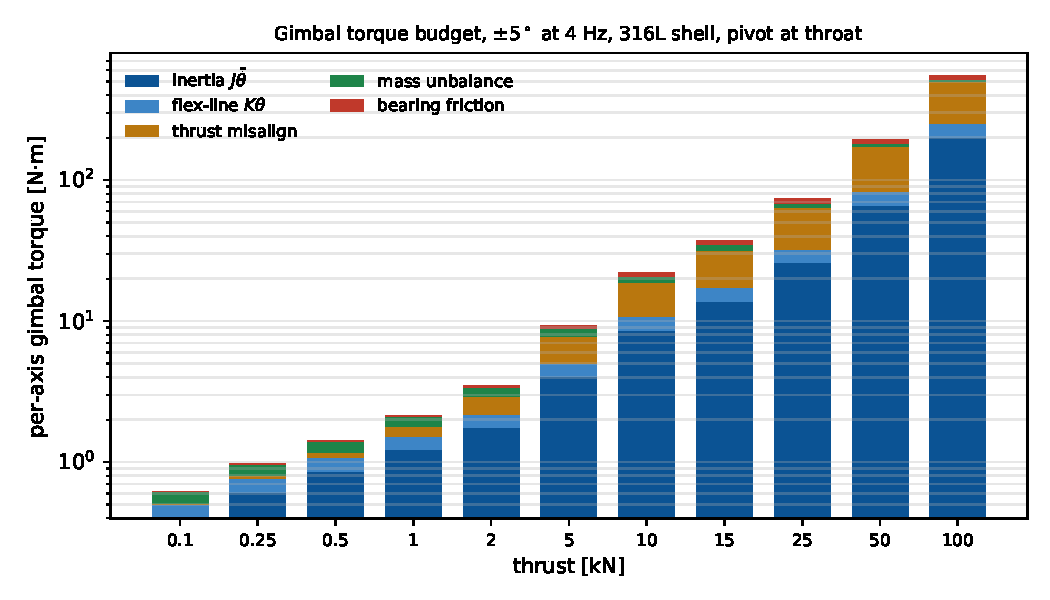
\includegraphics[width=\textwidth]{figures/tvc/budget.pdf}
\caption{Torque budget by term. Inertia dominates below $\sim$25\,kN;
above that the thrust-driven misalignment term overtakes it, because the
pivot-to-exit moment arm grows with the engine while the rate requirement
does not. At 100\,kN the split is misalignment 252\,N\,m, inertia 200\,N\,m,
flex line 50\,N\,m, friction 41\,N\,m, unbalance 11\,N\,m.}
\end{figure}

For a sanity check against flight hardware: the VINCI upper-stage gimbal
(a $\sim$180\,kN engine) used a friction-torque measurement rig with a
$300$\,N\,m range and $10$\,N\,m accuracy~\cite{neugebauer2006}. Our
100\,kN total sized requirement of $1109$\,N\,m against a friction
component of $41$\,N\,m is the right order for a rolling-element gimbal
at that scale.

% =====================================================================
\section{The actuator side}

\subsection{What a NEMA 17 actually delivers}

``NEMA 17'' is a \emph{frame size} ($42\times42$\,mm faceplate), not a
performance class. Across the common catalogue the holding torque spans
$16$--$79$\,N\,cm, i.e.\ $0.16$--$0.79$\,N\,m~\cite{stepperonline}. Three
things about that number matter here:

\begin{enumerate}[leftmargin=1.4em,itemsep=3pt]
\item \textbf{Holding torque is a standstill number.} It is what the motor
resists at zero speed with rated current. The torque available while
\emph{moving} follows the pull-out curve and falls with step rate as winding
inductance and back-EMF limit current rise. Datasheet pull-out curves for
42\,mm frames typically show useful torque collapsing through the
$600$--$1000$\,rpm region. This study uses $0.20$\,N\,m at $600$\,rpm for a
$0.45$\,N\,m motor and $0.35$\,N\,m at $600$\,rpm for a $0.79$\,N\,m motor
--- roughly $45\%$ of holding torque, which is a conventional and not
especially pessimistic derate.

\item \textbf{Rotor inertia is not negligible.} A 42\,mm frame carries
$J_{\text{rotor}} \approx 5.4\times10^{-6}$ to $1.4\times10^{-5}$\,kg\,m$^2$.
Section~\ref{sec:inertia} shows why this is the term that ends the argument.

\item \textbf{It is open loop.} The controller assumes the motor is where it
was told to go. When torque is momentarily inadequate the motor skips steps
and the controller does not know. Industrial guidance is explicit that this
disqualifies open-loop steppers from safety-critical positioning:
``should the machine snag on an object, [a servo] will be sensed
immediately\ldots\ and never lose position'', whereas an open-loop stepper
``does not know the actual location of the machine''~\cite{orientalmotor}.
A TVC actuator that silently loses $3^\circ$ of commanded gimbal is a
loss-of-vehicle event.
\end{enumerate}

\subsection{Gearing buys torque and sells speed; power is conserved}

The transmission ratio $N$ multiplies torque and divides speed. Mechanical
power passes through essentially unchanged (times efficiency $\eta$):
\begin{equation}
\tau_{\text{gimbal}} = N\eta\,\tau_{\text{motor}},\qquad
\omega_{\text{motor}} = N\,\omega_{\text{gimbal}},\qquad
P = \tau\omega \ \text{invariant.}
\end{equation}
For a screw-and-lever transmission with lead $L$ and moment arm $R$,
$N = 2\pi R/L$. A $60$\,mm arm on a $2$\,mm-lead screw gives $N = 188$;
on an $8$\,mm lead, $N = 47$.

This is why the power column of the results table is the most informative
single number in this report. Two NEMA 17s at $0.20$\,N\,m and $600$\,rpm
produce $2 \times 0.20 \times 62.8 = 25$\,W of shaft power. The requirement
is $9.4$\,W at $1$\,kN, $41$\,W at $5$\,kN, $97$\,W at $10$\,kN. No gearbox
changes those numbers.

\begin{figure}[H]\centering
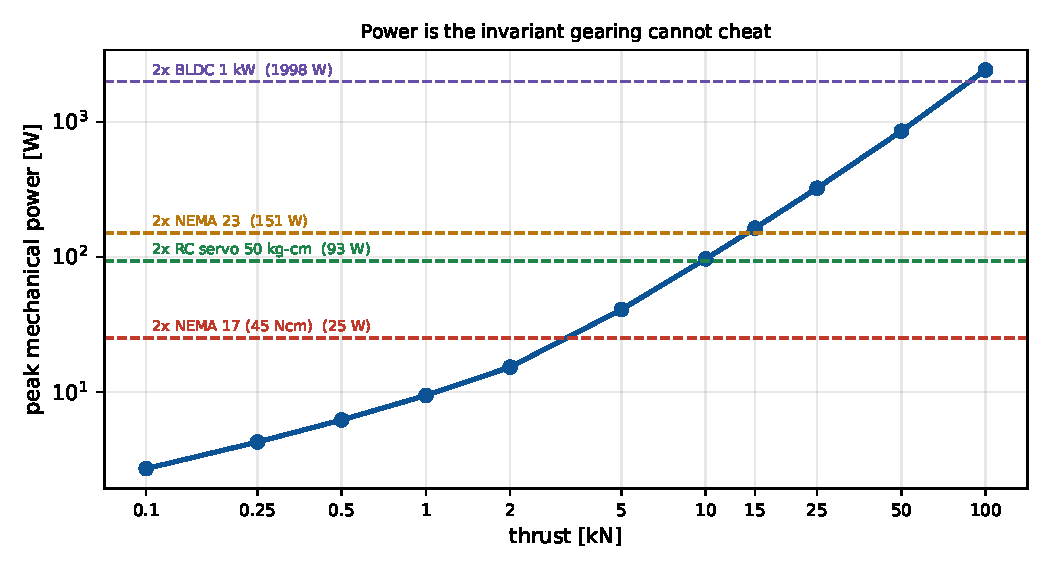
\includegraphics[width=\textwidth]{figures/tvc/power.pdf}
\caption{Required peak mechanical power per axis versus available shaft
power for four candidate actuator pairs. Crossings here are hard limits;
crossings on torque alone are not.}
\end{figure}

\subsection{Reflected inertia --- the term that kills high reduction}
\label{sec:inertia}

Referred to the gimbal axis, the motor's own rotor contributes
$N^2 J_{\text{rotor}}$ of apparent inertia. Because it scales as $N^2$ while
torque scales as $N$, past a certain ratio the motor spends more torque
accelerating itself than the engine. NASA MSFC found precisely this while
designing their second-generation EMTVC actuator:

\begin{keybox}
``Since inertia is a major concern due to the EMA's nature of operation,
optimization of horsepower, RPM, and motor rotor diameter is imperative.
\ldots\ Calculations show that the amount of inertia created by the rest of
the system is essentially negligible when compared to the inertia created by
the cyclic action of each rotor inertia.''
\hfill --- Cowan \& Weir, NASA MSFC~\cite{cowan1994}
\end{keybox}

Motion-control practice caps the load-to-rotor inertia ratio by device
class~\cite{orientalmotor}: about $10\times$ for an open-loop stepper,
$30\times$ for a closed-loop stepper, and $100\times$ for a true servo.
Inverting gives the ceiling
\begin{equation}
N_{\max}^{(J)} = \sqrt{\frac{k\,J_p}{J_{\text{rotor}}}},
\qquad k \in \{10,\,30,\,100\}.
\end{equation}
Worked at $1$\,kN with two $45$\,N\,cm NEMA 17s
($J_{\text{rotor}}=1.08\times10^{-5}$\,kg\,m$^2$ for the pair,
$J_p = 0.0221$\,kg\,m$^2$): $N_{\max}^{(J)} = 143$. Take instead the
$60$\,mm-arm / $2$\,mm-lead screw with $N = 188$ and the reflected rotor
inertia is $188^2 \times 1.08\times10^{-5} = 0.38$\,kg\,m$^2$ --- seventeen
times the engine it is supposed to be moving.

\subsection{The three screens}
\label{sec:screens}

Collecting the three requirements as bounds on $N$:
\begin{align}
\text{torque:}  &\quad N \geq N_{\min}^{(\tau)} = \frac{\tau_{\text{sized}}}{\eta\,\tau_{\text{motor}}}\\
\text{speed:}   &\quad N \leq N_{\max}^{(\omega)} = \frac{\omega_{\text{motor,max}}}{\omega_{\text{gimbal}}}\\
\text{inertia:} &\quad N \leq N_{\max}^{(J)} = \sqrt{k\,J_p / J_{\text{rotor}}}
\end{align}
The actuator is feasible iff
$N_{\min}^{(\tau)} \leq \min\!\left(N_{\max}^{(\omega)}, N_{\max}^{(J)}\right)$.
This is implemented in \cmd{screen\_actuator()} in
\cmd{scripts/tvc\_sizing\_study.py}, with $\eta = 0.85$.

% =====================================================================
\section{Verdict}

\subsection{Two NEMA 17s, directly answered}

\begin{table}[H]\centering\small
\caption{Feasible band in $N$ for two NEMA 17 (45\,N\,cm) steppers.
$N^\star$ is the geometric mid-band pick; ``margin'' is delivered torque
over required torque at $N^\star$.}
\begin{tabular}{r r r r r l}
\toprule
$F$ [kN] & $N_{\min}^{(\tau)}$ & $N_{\max}^{(\omega)}$ & $N_{\max}^{(J)}$ & $N^\star$ & verdict\\
\midrule
0.1 &   3.6 & 28.6 &  81.7 & 10.2 & \yes\ comfortable (margin 2.8)\\
0.5 &   8.3 & 28.6 & 120.2 & 15.4 & \yes\ (margin 1.86)\\
1   &  12.6 & 28.6 & 143.2 & 19.0 & \yes\ tight (margin 1.50)\\
2   &  20.5 & 28.6 & 171.6 & 24.2 & \yes\ marginal (margin 1.18)\\
5   &  54.8 & 28.6 & 259.8 & --- & \no\ band empty --- speed-limited\\
10  & 129.9 & 28.6 & 381.0 & --- & \no\\
25  & 433.7 & 28.6 & 659.0 & --- & \no\\
100 &3261.9 & 28.6 &1834.6 & --- & \no\\
\bottomrule
\end{tabular}
\end{table}

\begin{figure}[H]\centering
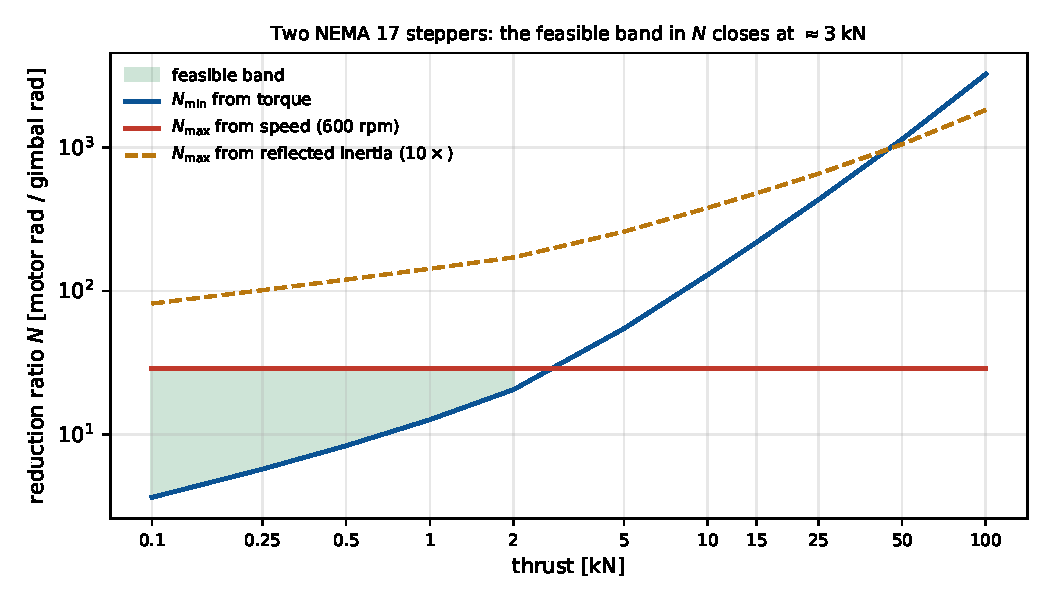
\includegraphics[width=\textwidth]{figures/tvc/nband.pdf}
\caption{The feasible band in reduction ratio for two NEMA 17s. The torque
floor rises with thrust; the speed ceiling is flat because the gimbal rate
requirement does not depend on engine size. They cross near 3\,kN.}
\end{figure}

Note what the crossing is \emph{not}: it is not the reflected-inertia limit
(the dashed line stays an order of magnitude above the torque floor
throughout the feasible region, and only meets it near 50\,kN where the
design has been infeasible for a decade of thrust already), and it is not
raw torque. It is that the stepper runs out of shaft speed. That is the physically interesting result,
and it is invisible if you only compare holding torque against required
torque.

\subsection{The map by thrust class}

\begin{figure}[H]\centering
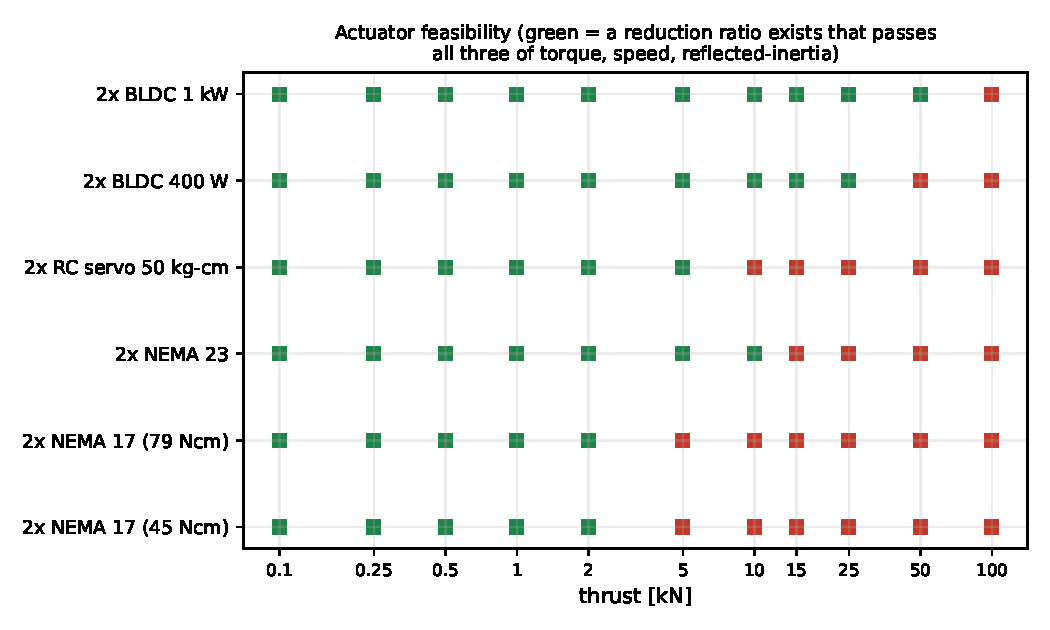
\includegraphics[width=\textwidth]{figures/tvc/feasibility.pdf}
\caption{Feasibility of six candidate actuator pairs across the sweep.}
\end{figure}

\begin{table}[H]\centering\small
\caption{Recommended actuation architecture by thrust class.}
\begin{tabular}{@{}p{2.3cm} p{4.6cm} p{7.4cm}@{}}
\toprule
\textbf{Class} & \textbf{Actuator} & \textbf{Why, and what to watch}\\
\midrule
\textbf{100--500\,N}\newline\small small
& 2$\times$ high-torque digital RC servo\newline (25--50\,kg\,cm, metal gear),\newline direct crank $N\approx1$--$2$
& $\tau_{\text{sized}} \leq 2.8$\,N\,m, $P \leq 6$\,W. Closed-loop by
construction, $\sim$$\$$45 each, and no gearbox to design. NEMA 17s also
close here but buy you nothing. Watch: servo gear backlash appears directly
as gimbal deadband.\\[3pt]
\textbf{1--10\,kN}\newline\small medium
& 2$\times$ brushless RC servo (50\,kg\,cm) to $\sim$7\,kN;\newline
2$\times$ NEMA 23 closed-loop, $N\approx20$--$35$, to 10\,kN;\newline
BLDC + planetary above that
& $\tau_{\text{sized}} = 4.3 \to 44$\,N\,m, $P = 9 \to 97$\,W. This is where
the choice actually matters. The NEMA 23 solution at 10\,kN closes with
margin $1.15$ --- too thin; prefer a 400\,W BLDC with a 20:1 planetary
(margin $>$5, $P_{\text{req}}/P_{\text{avail}} = 0.14$). Watch: at these
powers the flex-line spring rate must be \emph{measured}, not assumed.\\[3pt]
\textbf{$>$15\,kN}\newline\small large
& BLDC servo + roller screw, i.e.\ the MSFC EMTVC architecture in miniature;\newline
above $\sim$50\,kN, EMA/EHA/hydraulic
& $\tau_{\text{sized}} = 75 \to 1109$\,N\,m, $P = 164 \to 2432$\,W.
At 100\,kN even two 1\,kW BLDC servos fail ($P_{\text{req}}/P_{\text{avail}}
= 1.43$). Roller screws are specifically preferred over ball screws here for
start-transient shock capability~\cite{cowan1994}. Watch: this class needs a
real failure analysis --- ball/roller screw seizure is a
single-point-of-failure mode~\cite{bates2012}.\\
\bottomrule
\end{tabular}
\end{table}

\subsection{Why ``yes, below 3\,kN'' is still the wrong thing to build}

Even inside the feasible band, an open-loop stepper is a poor TVC actuator:

\begin{itemize}[leftmargin=1.4em,itemsep=2pt]
\item \textbf{Silent failure mode.} A skipped step is an unmeasured
position error, and the flight computer's estimate of the thrust vector is
now wrong in a way nothing detects~\cite{orientalmotor}.
\item \textbf{Torque margin is worst exactly when it matters.} Available
torque falls as speed rises; a large disturbance demands both simultaneously.
\item \textbf{Resonance.} Open-loop steppers have mid-band instability
regions; a lightly damped gimbal is a good place to find one.
\item \textbf{Holding current.} A stepper holds position by dissipating full
rated current at zero output power --- a poor thermal and battery choice for
a device that spends most of a burn near null.
\end{itemize}

If steppers are chosen anyway for cost or availability, add an encoder and
close the loop; that lifts the inertia ratio limit from $10\times$ to
$30\times$, raises usable speed, and removes the silent-failure mode.

% =====================================================================
\section{The 3D-printed demonstrator}

\subsection{Envelope}

\begin{table}[H]\centering\small
\caption{Print envelope against a Bambu Lab P1S ($256^3$\,mm, $240$\,mm
usable). Diameters include the 316L-equivalent wall.}
\begin{tabular}{r r r r r l}
\toprule
$F$ [kN] & $L$ [mm] & $D_{\text{exit}}$ & $D_{\text{cham}}$ & parts & note\\
\midrule
0.1  & 344 &  13.5 &  11.4 & 2 & split at flange\\
0.5  & 358 &  27.8 &  23.0 & 2 & split at flange\\
1    & 368 &  38.5 &  31.7 & 2 & \textbf{reference replica}\\
5    & 411 &  84.4 &  69.2 & 2 & split at flange\\
10   & 443 & 119.3 &  97.9 & 2 & split at flange\\
15   & 467 & 146.1 & 119.9 & 2 & split at flange\\
25   & 506 & 188.7 & 154.8 & 3 & split at flange\\
50   & 578 & 266.8 & 218.9 & 3 & exceeds bed diameter; print at $0.90\times$\\
100  & 679 & 377.3 & 309.6 & 3 & exceeds bed diameter; print at $0.64\times$\\
\bottomrule
\end{tabular}
\end{table}

Every case is length-limited, and for the same reason as
Section~\ref{sec:engine}: the $L^*$-driven chamber is thrust-independent.
Diagonal placement technically fits parts up to $443$\,mm but needs
full-height support against the one surface the demonstrator exists to show,
so it is not recommended.

\subsection{The 1\,kN reference replica}

\begin{figure}[H]\centering
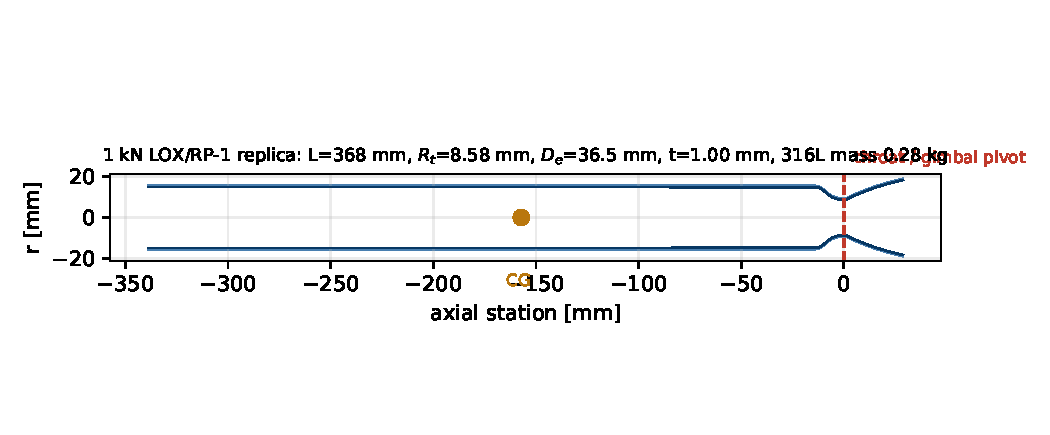
\includegraphics[width=\textwidth]{figures/tvc/contour1kn.pdf}
\caption{1\,kN LOX/RP-1 sea-level-matched contour with the hoop-sized wall,
throat/pivot station, and CG. The CG sits 157\,mm upstream of the pivot ---
that offset, not the shell's own inertia, is what the actuator fights.}
\end{figure}

\begin{table}[H]\centering\small
\begin{tabular}{@{}l l@{}}
\toprule
Throat radius & $8.58$\,mm\\
Exit diameter & $36.5$\,mm (outer $38.5$\,mm)\\
Chamber diameter & $29.7$\,mm (outer $31.7$\,mm)\\
Overall length & $368$\,mm\\
Wall thickness & $1.00$\,mm (hoop floor)\\
316L mass (if metal) & $0.280$\,kg\\
PLA mass (printed, $\rho=1240$) & $0.043$\,kg\\
Split & 2 parts at the chamber/converging flange, $\approx184$\,mm each\\
Print settings & 0.2\,mm layer, 3 walls, 15\% gyroid, no support with the\\
& nozzle printed exit-down (all overhangs $<45^\circ$ on the bell)\\
Estimated time & $\sim$6--8\,h per half at 0.2\,mm on a P1S\\
\bottomrule
\end{tabular}
\end{table}

Print it in \textbf{PETG or ASA}, not PLA. The arXiv hobby-gimbal study moved
from PLA to ABS for exactly this reason --- PLA's low glass transition made
sustained operation near the motor a concern, and ABS is both less dense
($1.04$ vs $1.24$\,g/cm$^3$) and tougher~\cite{singh2025}. The P1S is
enclosed, so ASA/ABS is a reasonable choice on this printer specifically.

\subsection{The gimbal ring, and what the demo proves}

Build the two-axis ring around the throat station, not the chamber: that puts
the pivot where the analysis puts it and keeps $J_p$ at the value the torque
budget assumed. Two orthogonal pivot axes, actuator horns at a
$50$--$70$\,mm arm, and hard stops at $\pm6^\circ$.

\begin{warnbox}
\textbf{Be precise about what the demonstrator does and does not show.}
A PLA/PETG replica has $\sim$$15\%$ of the steel mass and therefore
$\sim$$15\%$ of the inertia. It \emph{does} validate: kinematics, actuator
travel and interference, control-loop tuning topology, sensor integration,
mechanism backlash, and the gimbal-ring geometry. It \emph{does not} validate
any torque, rate, or power number in this report. To make the bench test
quantitative, ballast the printed part to the 316L wet mass \emph{and} match
$J_p$ --- matching mass alone is not sufficient, because the parallel-axis
term dominates and depends on where you put the ballast.
\end{warnbox}

% =====================================================================
\section{Bringing TVC into LREKit: a \texttt{raosim/tvc.py} module}

The analysis above is currently a script that post-processes
\cmd{contour.csv}. Everything it needs already exists inside LREKit; the
natural next step is to make it a first-class module so that any design point
the CLI produces carries a TVC verdict.

\subsection{What already exists and what is missing}

\begin{table}[H]\centering\small
\begin{tabular}{@{}p{4.7cm} p{4.0cm} p{6.2cm}@{}}
\toprule
\textbf{Needed} & \textbf{Status} & \textbf{Where}\\
\midrule
Wall contour $(x, r)$ & \textbf{present} & \cmd{design\_nozzle\_v2} $\to$ \cmd{contour.csv}\\
Wall thickness, station-wise & \textbf{present} & \cmd{thermal\_design.py}, \cmd{regen\_profile.py}\\
Material density and $S_y$ & \textbf{present} & \cmd{materials.py}\\
Enclosed solid volume & \textbf{present} & \cmd{export.py} STL diagnostics\\
Injector/valve/manifold mass & \emph{partly} & \cmd{injector\_cad.py} has geometry, not mass\\
Pump/battery mass & \textbf{present} & \cmd{pumps.py}, \cmd{mdo/pump.py}\\
\textbf{Mass properties (CG, $J$)} & \textbf{missing} & --- this module\\
\textbf{Gimbal torque budget} & \textbf{missing} & --- this module\\
\textbf{Actuator screen} & \textbf{missing} & --- this module\\
Flex-line spring rate & \textbf{missing, and not predictable} & must be a user input or a measured table\\
\bottomrule
\end{tabular}
\end{table}

\subsection{Proposed interface}

\begin{lstlisting}[language=Python]
# raosim/tvc.py

@dataclass(frozen=True)
class MassProperties:
    mass_kg: float
    x_cg_m: float
    I_transverse_cg: float
    I_transverse_pivot: float
    pivot_x_m: float
    components: dict[str, float]   # shell / jacket / injector / trapped prop

def mass_properties(contour, thickness, material, *,
                    pivot="throat", extras=()) -> MassProperties: ...

@dataclass(frozen=True)
class GimbalRequirement:
    theta_max_deg: float = 5.0
    bandwidth_hz: float = 4.0        # SSME envelope, NTRS 19940025147
    k_flex_nm_per_rad: float | None = None   # None -> reported as UNPINNED
    mu_bearing: float = 0.003
    misalignment_deg: float = 0.5
    vehicle_accel_g: float = 4.0
    design_margin: float = 2.0

def torque_budget(mp, thrust_n, req) -> TorqueBudget: ...
def screen_actuators(budget, catalog=ACTUATORS) -> list[Screen]: ...
\end{lstlisting}

\subsection{CLI surface and output contract}

\begin{lstlisting}
--tvc                          enable the TVC block
--tvc-deflection 5.0           [deg]
--tvc-bandwidth 4.0            [Hz]
--tvc-pivot throat|injector|cg|<x in m>
--tvc-flex-stiffness <N.m/rad> measured; omit to report the term unpinned
--tvc-actuator-catalog <json>  override the built-in candidate list
--tvc-dry-mass-extras <json>   injector/valve/manifold masses
\end{lstlisting}

and a \cmd{summary.json} block:

\begin{lstlisting}
"tvc": {
  "mass_properties": {"mass_kg":..., "x_cg_m":..., "I_pivot_kgm2":...,
                      "pivot_x_m":..., "components":{...}},
  "requirement":     {"theta_max_deg":5.0, "bandwidth_hz":4.0, ...},
  "torque_budget":   {"inertia":..., "flex":..., "friction":...,
                      "misalignment":..., "unbalance":...,
                      "total":..., "sized":..., "peak_power_w":...},
  "actuators":       [{"name":..., "feasible":true, "N_band":[lo,hi],
                       "binding":"speed", "margin":1.50}, ...],
  "gates": {"flex_stiffness_pinned": false,
            "moment_arm_model_valid": true,
            "any_actuator_feasible": true}
}
\end{lstlisting}

\paragraph{Release gates.} The repository's convention is that a physically
unqualified number must be gated, not quietly reported. Three gates belong
here:
\begin{enumerate}[leftmargin=1.4em,itemsep=2pt]
\item \texttt{flex\_stiffness\_pinned} --- \textsc{fail} unless
\cmd{--tvc-flex-stiffness} was supplied from measurement. The $25\%$-of-inertia
placeholder used in this report is a screening assumption and must never pass
as literature.
\item \texttt{moment\_arm\_model\_valid} --- \textsc{warn} above
$\theta_{\max} > 5^\circ$, where the planar moment-arm relation starts to
degrade~\cite{stepp2024}.
\item \texttt{actuator\_open\_loop} --- \textsc{warn} whenever the selected
candidate is an open-loop stepper, regardless of margin.
\end{enumerate}

% =====================================================================
\section{The traditional solver and the MDO: what each one is}
\label{sec:solver-vs-mdo}

This section answers the three questions directly: what the traditional
solver does, what the MDO does that it cannot, and whether the MDO is
supposed to be part of the traditional solver.

\subsection{The traditional solver: a forward analysis pipeline}

\cmd{raosim/run\_nozzle.py} (roughly 3300 lines, reached by
\cmd{python -m raosim}) is a \textbf{sequential forward analysis}. You give
it a complete specification --- $P_c$, $\varepsilon$, target thrust, $L^*$,
contraction ratio, channel geometry, pintle diameter, coolant, materials ---
and it walks a fixed chain:

\begin{center}
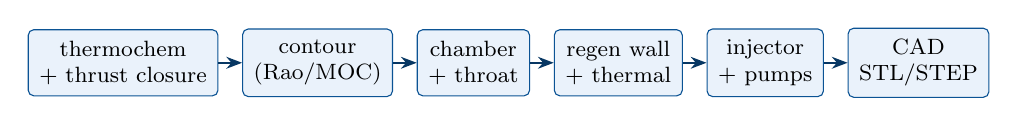
\begin{tikzpicture}[node distance=3mm, every node/.style={font=\footnotesize},
  box/.style={draw=accent,fill=notebg,rounded corners=2pt,inner sep=4pt,
              minimum height=7mm,align=center},
  ar/.style={-{Stealth[length=2mm]},draw=accentdark,thick}]
\node[box] (a) {thermochem\\+ thrust closure};
\node[box,right=of a] (b) {contour\\(Rao/MOC)};
\node[box,right=of b] (c) {chamber\\+ throat};
\node[box,right=of c] (d) {regen wall\\+ thermal};
\node[box,right=of d] (e) {injector\\+ pumps};
\node[box,right=of e] (f) {CAD\\STL/STEP};
\draw[ar] (a)--(b); \draw[ar] (b)--(c); \draw[ar] (c)--(d);
\draw[ar] (d)--(e); \draw[ar] (e)--(f);
\end{tikzpicture}
\end{center}

Its properties:
\begin{itemize}[leftmargin=1.4em,itemsep=2pt]
\item \textbf{One direction.} Information flows left to right. If the wall
sizing comes back infeasible, nothing upstream changes --- the run reports
the failure and stops. \emph{You} are the optimiser.
\item \textbf{Highest-fidelity models.} This is where the exact variational
Rao solve, method-of-characteristics, station-wise thermostructural wall
sizing, machined-pintle CAD, and pump B-reps live.
\item \textbf{It is where artifacts come from.} STL, STEP, contour CSV,
manufacturing reports. The MDO layer produces none of these.
\item \textbf{Local coupling only.} A few loops are closed internally (the
spray$\to$$c^*$ fixed point, the channel-height sweep), but the disciplines
are not solved simultaneously.
\end{itemize}

\subsection{The MDO: a coupled, differentiable, inverse solve}

\cmd{raosim/mdo/} is a different \emph{kind} of object. Its own package
docstring calls it ``a pure-numerical layer: no CAD, no file I/O in the
differentiated path''. It does two things the forward pipeline structurally
cannot:

\paragraph{(1) It closes the couplings simultaneously (MDF).}
\cmd{engine.py:solve\_engine} evaluates every block --- nozzle, cooling,
injector, pump/battery --- as one coupled residual $R(y, x) = 0$ and solves
it with Newton, so the cooling $\Delta p$ that the pump must supply and the
pump discharge pressure that the cooling channels see are consistent at the
solution rather than after a couple of hand iterations. Sensitivities come
from the \emph{implicit function theorem}, never from unrolling the solver:
\begin{equation}
\pd{y}{x} = -\left(\pd{R}{y}\right)^{-1}\pd{R}{x}.
\end{equation}

\paragraph{(2) It inverts the question.}
The forward solver answers ``given this design, is it feasible?''.
\cmd{nlp.py} answers ``\emph{find} the design that minimises feed-system mass
subject to $I_{sp} \geq$ floor and all 17 constraints''. It is an
$\varepsilon$-constraint NLP over a 10-variable unit box with exact JAX
Jacobians handed to SLSQP, and it can trace a Pareto frontier rather than
returning one point.

The 10 design variables are $P_c$, $\varepsilon$, the two injector $\Delta p$
fractions, pintle diameter, pump rpm, channel width and height, film-cooling
fraction, and wall thickness. The 17 constraints span separation, coking,
channel fit, chug, pintle transition branch, pump suction and tip speed,
aspect ratio, blockage band, structural stress, wall temperature, film
capacity, property-table domain, Rao-chart domain, and wall monotonicity.

\subsection{Is the MDO part of the traditional solver?}

\begin{keybox}
\textbf{No --- and it is not a replacement either.} They are two independent
front ends over a shared physics vocabulary, joined by an explicit bridge.
The MDO \emph{searches}; the traditional solver \emph{resolves and builds}.
The guide states the relationship plainly: ``The traditional nozzle/CAD
workflow is still the default.''
\end{keybox}

Concretely, the two live side by side on the same CLI:
\begin{lstlisting}
lrekit                                   # traditional forward workflow (default)
lrekit --engine-mdo        --pc 3e6 ...  # one coupled MDO point evaluation
lrekit --engine-mdo-optimize --isp-min 200   # the constrained optimisation
\end{lstlisting}

and are connected by two contracts:
\begin{itemize}[leftmargin=1.4em,itemsep=2pt]
\item \cmd{mdo/snapshot.py} --- \texttt{EngineAnalysisSnapshot}, a versioned
description of an analysed engine that \emph{both} sides can emit
(\texttt{snapshot\_from\_mdo}, \texttt{snapshot\_from\_traditional}) and that
\texttt{compare\_snapshots} can diff.
\item \cmd{mdo/postprocess.py} --- the Phase-11 bridge. It maps an optimised
\texttt{EngineState} back into a \texttt{design\_nozzle\_v2} input, pins the
exact chamber thermochemistry so the two sides cannot silently drift apart,
re-evaluates at higher fidelity, and emits a \textbf{parity report}.
\end{itemize}

The reason the bridge exists is that the two sides deliberately do not use
the same nozzle model. The MDO's \cmd{grid.py} uses the analytic Rao/TOP
approximation --- fast, differentiable, piecewise-$C^1$ --- because a full
variational Rao solve inside an SLSQP inner loop would be intractable. The
authoritative post-optimum contour then comes from
\cmd{design\_nozzle\_v2}. The parity report is what keeps that substitution
honest.

\subsection{What the MDO does that the traditional solver cannot}

\begin{table}[H]\centering\small
\begin{tabular}{@{}p{4.0cm} p{5.2cm} p{5.6cm}@{}}
\toprule
& \textbf{Traditional solver} & \textbf{MDO layer}\\
\midrule
Question answered & ``is this design feasible, and what does it look like?'' & ``what is the best feasible design?''\\
Direction & forward analysis & inverse / optimisation\\
Coupling & sequential, a few local fixed points & simultaneous (MDF), Newton + IFT\\
Derivatives & none & exact, by JAX AD through the implicit solve\\
Constraints & checked and reported after the fact & \emph{enforced} by the NLP, all 17\\
Trade studies & one run per point, by hand & Pareto frontier in one call\\
Fidelity & highest (exact Rao, MOC, station-wise wall) & reduced, differentiable surrogates\\
Artifacts & STL, STEP, CSV, reports & none --- numbers only\\
Backend & NumPy or JAX & JAX only\\
\bottomrule
\end{tabular}
\end{table}

The distinction that matters most: \textbf{gradients}. Without them, exploring
a 10-dimensional design space against 17 constraints means finite differences
--- at minimum 11 forward solves per gradient, each of which is a full
Newton-converged coupled engine. With the implicit function theorem it is one
solve plus one linear system. That is what turns ``run a parameter sweep
overnight'' into ``optimise in a few minutes'', and it is the whole reason
the MDO layer is written in JAX rather than being another mode of
\cmd{run\_nozzle.py}.

The second distinction: \textbf{the MDO can find couplings you would not
think to check by hand.} The film-cooling fraction is simultaneously a
coking lever, an $I_{sp}$ penalty, a coolant-flow change, and therefore a
pump-power and battery-mass change. A human sweeping one variable at a time
will not land on the joint optimum. A gradient will.

% =====================================================================
\section{Adding TVC to the MDO}
\label{sec:mdo-tvc}

Once \cmd{raosim/tvc.py} exists on the traditional side, moving it into the
MDO is the interesting part --- because TVC is exactly the kind of
constraint that couples to variables you would not expect.

\subsection{Why it belongs in the MDO at all}

The actuator requirement is driven by $J_p$, which is driven by chamber
length and wall thickness, which are driven by $L^*$, contraction ratio,
$P_c$, and the thermostructural wall sizing. Every one of those is either
already an MDO design variable or one step away from it. Section~\ref{sec:engine}
showed the specific consequence: at low thrust the $L^*$-driven chamber
length, not the wall mass, sets the actuator size. A designer optimising
for $I_{sp}$ and feed mass alone will happily choose a long chamber and hand
the TVC engineer a bill they never see.

\subsection{Three ways in, in increasing order of ambition}

\paragraph{(a) As a reported output only.} Add $J_p$, $\tau_{\text{sized}}$,
and $P_{\text{peak}}$ to \texttt{EngineState} and report them. Zero risk,
no new design variables, and immediately useful --- you can read the TVC
cost of every point on an existing Pareto frontier.

\paragraph{(b) As a hard constraint.} Add
\begin{equation}
g_{\text{tvc}}(x) = 1 - \frac{\tau_{\text{sized}}(x)}{\tau_{\text{actuator}}} \geq 0
\end{equation}
to \texttt{CONSTRAINT\_NAMES} and \texttt{DEFAULT\_ENFORCED}, with
$\tau_{\text{actuator}}$ a mission input. This says ``design me the best
engine that my chosen actuator can actually gimbal''. It is the formulation
that matches how a real vehicle programme works, because the actuator is
usually selected before the engine is frozen.

\paragraph{(c) As a mass term in the objective.} The existing objective is
smooth electric-feed mass. Adding actuator and gimbal-structure mass ---
both of which scale with $\tau_{\text{sized}}$ --- makes the optimiser trade
chamber length against actuator mass on its own. This is the most valuable
and the most delicate, because it needs an actuator mass-versus-torque
scaling law that is honest. That law should come from a fitted catalogue
with its fit residual reported, not from a guess.

\subsection{What has to be true for it to work}

\begin{table}[H]\centering\small
\begin{tabular}{@{}p{4.2cm} p{10.6cm}@{}}
\toprule
\textbf{Requirement} & \textbf{How to satisfy it}\\
\midrule
Differentiable, no branches
& The mass integral is a smooth quadrature over the station grid --- fine. The
\emph{screen} is not: \texttt{min}, \texttt{max}, and the feasibility
predicate are non-smooth. Put the screen in post-processing and expose only
the smooth $\tau_{\text{sized}}(x)$ to the NLP.\\[3pt]
Fixed shapes, no Python control flow
& \cmd{mdo/grid.py} already gives a fixed-topology station grid; integrate on
it directly rather than on the variable-length \cmd{contour.csv}.\\[3pt]
No zero Jacobian columns
& The guide's own dead-variable check (§8) must be re-run after adding the
constraint. If $\partial g_{\text{tvc}}/\partial x_k = 0$ for every $k$, the
constraint is decoration.\\[3pt]
A NumPy oracle + parity test
& Repository rule: every JAX block keeps a NumPy oracle.
\cmd{scripts/tvc\_sizing\_study.py} as written \emph{is} that oracle --- it is
pure Python/NumPy. Add \cmd{tests/test\_mdo\_tvc.py} asserting parity to
$10^{-8}$.\\[3pt]
Snapshot round-trip
& Add the TVC block to \texttt{EngineAnalysisSnapshot} so
\texttt{compare\_snapshots} covers it and MDO/traditional cannot drift.\\
\bottomrule
\end{tabular}
\end{table}

\subsection{What I expect it to change}

A concrete, falsifiable prediction: with (b) or (c) enabled at the 1\,kN
scale, the optimiser should push \emph{down} on chamber length --- higher
contraction ratio at fixed $L^*$, or a lower $L^*$ where combustion
efficiency permits --- because $J_p$ is dominated by the
$m\,d_{\text{cg}}^2$ parallel-axis term. That would trade a small $c^*$
efficiency loss against a large actuator saving, and it is precisely the
kind of trade the forward solver cannot find because $L^*$ and actuator
torque never meet in the same calculation. If the optimiser does \emph{not}
do this, the constraint is probably not wired to the variables it should be,
and the dead-column check above will say so.

% =====================================================================
\section{Limitations}

Stated plainly, because a portfolio piece that overclaims is worse than one
that is narrow and honest:

\begin{enumerate}[leftmargin=1.4em,itemsep=3pt]
\item \textbf{The flex-line spring rate is a placeholder.} $25\%$ of the
inertia term is a screening assumption with no source. On real engines this
term is measured. It could plausibly be $2\times$ larger, which would move
the NEMA 17 crossover from $\sim$3\,kN to $\sim$2\,kN. This is the single
largest uncertainty in the report.
\item \textbf{Stepper pull-out torque is a derate, not a measurement.}
$45\%$ of holding torque at $600$\,rpm is conventional but motor-, driver-,
and bus-voltage-specific. A $48$\,V driver on a low-inductance winding does
considerably better than a $12$\,V one.
\item \textbf{Only the shell is integrated.} Injector, valves, manifolds and
trapped propellant enter through a single $2.2\times$ factor. A real design
would integrate them individually --- and their mass sits near the injector
end, i.e.\ at large $d_{\text{cg}}$, so this factor is doing more work than
its simplicity suggests.
\item \textbf{Contours are seed geometry.} Runs used
\texttt{--max-nfev 0}, so the contours are the analytic Rao/TOP seed, not the
converged variational solve. Mass properties are insensitive to that at the
percent level; performance numbers would not be.
\item \textbf{No structural dynamics.} The gimbal ring, actuator mounts, and
vehicle backstructure have modes. The published rule of thumb is to keep the
closed-loop bandwidth below one tenth of the backstructure mode frequency;
the MSFC test article showed load-structure resonance at $8$--$9$\,Hz against
a $4$\,Hz bandwidth~\cite{cowan1994}. Nothing here models that.
\item \textbf{No thermal environment on the actuator.} Radiation from a
316L nozzle at $1000$\,K is not modelled and is a real constraint on
where the actuators can be mounted.
\end{enumerate}

% =====================================================================
\section{Reproducing this}

\begin{lstlisting}
# 1. generate contours (one per thrust point)
for F in 100 250 500 1000 2000 5000 10000 15000 25000 50000 100000; do
  PYTHONPATH=. python -m raosim --no-banner --backend numpy \
    --propellant LOX/RP-1 --oxidizer LOX --fuel RP-1 \
    --pc 3.0e6 --target-thrust $F --epsilon 4.524 --pa-over-p0 0.033775 \
    --length-pct 80 --l-star 1.0 --contraction-ratio 3.0 \
    --minimum-cylindrical-length 0.03 --ru-factor 1.5 \
    --max-nfev 0 --n-control 8 --n-kernel 12 \
    --material 316l --out builds/tvc/F$F
done

# 2. run the sizing study
python scripts/tvc_sizing_study.py --contours builds/tvc \
       --json builds/tvc/study.json --theta 5 --bandwidth 4
\end{lstlisting}

% =====================================================================
\begin{thebibliography}{99}
\small

\bibitem{cowan1994} J.~R. Cowan and R.~A. Weir,
``Design and Test of Electromechanical Actuators for Thrust Vector Control,''
NASA George C. Marshall Space Flight Center, NTRS 19940025147.
\url{https://ntrs.nasa.gov/api/citations/19940025147/downloads/19940025147.pdf}
\emph{(SSME 4\,Hz / 20--25$^\circ$ bandwidth requirement; rotor-inertia
dominance; roller-screw selection.)}

\bibitem{bates2012} L.~B. Bates and D.~T. Young,
``Developmental Testing of Electric Thrust Vector Control Systems for Manned
Launch Vehicle Applications,'' \emph{Proc. 41st Aerospace Mechanisms
Symposium}, JPL, May 2012. NASA MSFC, NTRS 20120014541.
\url{https://ntrs.nasa.gov/api/citations/20120014541/downloads/20120014541.pdf}
\emph{(TVC reacts against inertia, gimbal/flex-bearing stiffness, structure
and propellant flex lines; EMA/EHA/IAP architectures; ball-screw
single-point-of-failure.)}

\bibitem{stepp2024} N.~A. Stepp,
``MSFC-TVC $|$ TB-03: Derivation of Thrust Vector Control (TVC)
Actuator-Force / Gimbal-Torque Transformation Matrix,''
NASA/TM--20240012525, Marshall Space Flight Center, December 2024.
\url{https://ntrs.nasa.gov/citations/20240012525}
\emph{(Planar moment-arm relation degrades beyond 2--3$^\circ$; $\approx$2\%
error at 15$^\circ$ yaw in the worked example.)}

\bibitem{neugebauer2006} C.~Neugebauer, M.~Falkner, L.~Supper and G.~Traxler,
``Bearing Development for a Rocket Engine Gimbal,''
\emph{Proc. 38th Aerospace Mechanisms Symposium}, ESMATS, 2006.
\url{https://esmats.eu/amspapers/pastpapers/pdfs/2006/neugebauer.pdf}
\emph{(VINCI upper-stage gimbal; rolling bearings chosen for low friction
torque; 300\,N\,m friction measurement range, 10\,N\,m accuracy;
$\pm6^\circ$ development test range.)}

\bibitem{singh2025} E.~Singh,
``Design and Testing of a Low-Cost 3D-Printed Servo Gimbal for Thrust Vector
Control in Model Rockets,'' arXiv:2509.00061, August 2025.
\url{https://arxiv.org/abs/2509.00061}
\emph{($\pm5^\circ$ deflection, 44.5\,ms mean response with SG90 servos,
30\,N thrust load, PLA$\to$ABS material change and its rationale.)}

\bibitem{orientalmotor} Oriental Motor,
``The Choice Between Servo Motors and Stepper Motors.''
\url{https://blog.orientalmotor.com/the-choice-between-servo-motors-and-stepper-motors}
\emph{(Load-to-rotor inertia ratios: $\sim$10$\times$ open-loop stepper,
$\sim$30$\times$ closed-loop stepper, $\sim$100$\times$ servo; open-loop
step-loss failure mode.)}

\bibitem{stepperonline} StepperOnline (OMC),
NEMA 17 hybrid stepper motor catalogue and datasheets.
\url{https://www.omc-stepperonline.com/nema-17-stepper-motor}
\emph{(Holding torque 16--79\,N\,cm across the 42\,mm frame; rotor inertia,
rated current, and physical dimensions used in the actuator catalogue.)}

\bibitem{sutton} G.~P. Sutton and O.~Biblarz,
\emph{Rocket Propulsion Elements}, 9th ed., Wiley, 2017.
\emph{(LOX/RP-1 chamber gas properties, Table 5-5, as used by
\cmd{raosim/propellants.py}; gimbal TVC as the dominant large-vehicle
method.)}

\bibitem{sp125} NASA SP-125,
\emph{Design of Liquid Propellant Rocket Engines}.
\emph{(Characteristic length $L^*$ = 40--50\,in for LOX/RP-1, Table 4-1;
stainless steel named as a common thrust-chamber wall metal, p.~105;
station-wise liner stress screens, eqs.~4-28/29/31/32 --- all as cited
inside LREKit's own source.)}

\bibitem{sp8120} NASA SP-8120,
\emph{Liquid Rocket Engine Nozzles}.
\emph{(Throat-approach radius-ratio bounds and the Rao/TOP chart domain
enforced by \cmd{raosim/throat\_geometry.py}.)}

\bibitem{lrekit} I.~Shahid, \emph{LREKit / RaoRocketSim}.
Modules cited directly: \cmd{raosim/materials.py} (316L catalogue entry),
\cmd{raosim/run\_nozzle.py} (traditional workflow),
\cmd{raosim/mdo/} (\cmd{engine.py}, \cmd{nlp.py}, \cmd{snapshot.py},
\cmd{postprocess.py}), \cmd{docs/MDO\_GUIDE.md},
\cmd{scripts/tvc\_sizing\_study.py} (added by this study).

\end{thebibliography}

\end{document}
